\chapter{Introduction} \label{cap:cap1}

\section{Purpose}
The purpose of this document is to present the cost estimation for the WheaterCal system. It will estimate the effort required and the costs for the analisys and the development of the application using, respectively, the UFP and COCOMO II methods.
This document is intended for both the stakeholders and the developers of the system.
Stakeholders of the system are the client, which is our teacher and their assistants, composing the group that will evaluate our project, the testers, which are a team with our same project and our same tasks and the developers, which are the authors of this document.

\bibliographystyle{ieeetr}
\begin{thebibliography}{9}
\bibitem{1} 
Center for Systems and Software Engineering,
\textit{\href{http://csse.usc.edu/tools/COCOMOII.php}{COCOMO II online estimation tool}},
Ray Madachy
 
\bibitem{2} 
Paolo Polidori, Marco Edemanti,
\textit{Design Document for WeatherCal project},
2014.
 
\bibitem{3} 
Paolo Polidori, Marco Edemanti,
\textit{Requirement analisys and specification document for WeatherCal project},
2014.
\end{thebibliography}

\chapter{UFP effort estimation}

\section{Estimation}
\subsection{ILF Internal Logic Files}
\begin{tabularx}{\linewidth}{|X|c|c|}
  \hline \b{File name} & \b{Weight} & \b{FPs}\\
  \hline Calendar & Simple & 7 \\
  \hline Event & Complex & 15 \\
  \hline Ownership & Simple & 7 \\
  \hline User & Simple & 7 \\
  \hline Participation & Simple & 7 \\
  \hline User group & Simple & 7 \\
  \hline Weather value constraint & Simple & 7 \\
  \hline Weather state constraint & Simple & 7 \\
  \Xhline{4\arrayrulewidth} \multicolumn{2}{|l|}{Total}  & 64 \\
  \hline
\end{tabularx}
\subsection{EIF External Interface Files}
\begin{tabularx}{\linewidth}{|X|c|c|}
  \hline \b{File name} & \b{Weight} & \b{FPs}\\
  \hline OpenWeatherMap & Medium & 7 \\
  \hline Google Timezone & Simple & 5 \\
  \hline Google Maps & Simple & 5 \\
  \Xhline{4\arrayrulewidth} \multicolumn{2}{|l|}{Total}  & 17 \\
  \hline
\end{tabularx}
\subsection{EI External Inputs}
\begin{tabularx}{\linewidth}{|X|c|c|}
  \hline \b{File name} & \b{Weight} & \b{FPs}\\
  \hline Login & Simple & 3 \\
  \hline Logout & Simple & 3 \\
  \hline Sign in & Medium & 4 \\
  \hline Manage participation & Simple & 3 \\
  \hline Create event & Complex & 6 \\
  \hline Edit event & Complex & 6 \\
  \hline Delete event & Simple & 3 \\
  \hline Invites management & Complex & 6 \\
  \hline User search & Complex & 6 \\
  \Xhline{4\arrayrulewidth} \multicolumn{2}{|l|}{Total}  & 40 \\
  \hline
\end{tabularx}
\subsection{EIQ External Inquiries}
\begin{tabularx}{\linewidth}{|X|c|c|}
  \hline \b{File name} & \b{Weight} & \b{FPs}\\
  \hline Personal schedule & Complex & 6 \\
  \hline Notifications & Complex & 6 \\
  \hline Other users' schedule & Simple & 3 \\
  \hline Local weather info & Medium & 4 \\
  \hline Bad weather notification (owner) & Complex & 6 \\
  \hline Bad weather notification (participant) & Medium & 4 \\
  \Xhline{4\arrayrulewidth} \multicolumn{2}{|l|}{Total}  & 29 \\
  \hline
\end{tabularx}
\subsection{EO External Outputs}
Since there are no external outputs in our system, no FPs will be added.

\subsection{Summary}
The total FPs for the project are \(64+17+40+29+0=150\). The number of source line code is so \(150*50=7500\). We used 50 as SLOC/FP factor as an average among J2EE (46), Java (53) and Javascript (47).

\section{Comparison with actual values}
From the UFP estimation we resulted in having to develop a \(7,5\) KLOC, which is pretty close to the reality:\\
\begin{tabularx}{\linewidth}{|X|c|c|c|c|}
  \hline \b{Language} & \b{files} & \b{blank} & \b{comment} & \b{code}\\
  \Xhline{4\arrayrulewidth}Javascript & 12 & 29 & 108 & 468\\
  \hline Java & 53 & 842 & 860 & 4568\\
  \hline CSS & 5 & 110 & 43 & 1367\\
  \hline JavaServer Faces & 4 & 46 & 2 & 821\\
  \hline XML & 10 & 1 & 22 & 255\\
  \hline HTML & 4 & 0 & 0 & 94\\
  \hline Maven & 1 & 0 & 182 & 93\\
  \hline SQL & 1 & 0 & 0 & 1\\
  \Xhline{4\arrayrulewidth} SUM & 100 & 1028 & 1217 & 7667\\
  \hline
\end{tabularx}\\

\chapter{COCOMO II cost estimation}
\section{Software evalutaion}
We can use the SLOC number obtained using the UFP method for estimating the COCOMO costs. We derived the scale drivers and the cost drivers using the tool referenced at \cite{1}.\\


\begin{tabularx}{\linewidth}{|X|c|}
\hline \multicolumn{2}{|l|}{\b Software Development (Elaboration and Construction)}\\
\Xhline{4\arrayrulewidth} Effort & 26.4 Person-months\\
\hline Schedule & 14.1 Months\\
\hline
\end{tabularx}\\

\begin{tabularx}{\linewidth}{|X|c|c|c|}
\hline \multicolumn{4}{|l|}{\b Acquisition Phase Distribution}\\
\Xhline{4\arrayrulewidth} \b{Phase} & \b{Effort (Person-months)} & \b{Schedule (Months)} & \b{Average Staff}\\
\Xhline{4\arrayrulewidth} Inception & 1.6 & 1.8 & 0.9\\
\hline Elaboration & 6.3 & 5.3 & 1.2\\
\hline Construction & 20.1 & 8.8 & 2.3\\
\hline Transition & 3.2 & 1.8 & 1.8\\
\hline
\end{tabularx}\\

\begin{tabularx}{\linewidth}{|X|c|c|c|c|}
\hline \multicolumn{5}{|l|}{\b Software Effort Distribution for RUP/MBASE (Person-Months)}\\
\Xhline{4\arrayrulewidth} \b{Phase/Activity} & \b{Inception} & \b{Elaboration} & \b{Construction} & \b{Transition}\\
\Xhline{4\arrayrulewidth} Management & 0.2 & 0.8 & 2.0 & 0.4\\
\hline Environment/CM & 0.2 & 0.5 & 1.0 & 0.2\\
\hline Requirements & 0.6 & 1.1 & 1.6 & 0.1\\
\hline Design & 0.3 & 2.3 & 3.2 & 0.1\\
\hline Implementation & 0.1 & 0.8 & 6.8 & 0.6\\
\hline Assessment & 0.1 & 0.6 & 4.8 & 0.8\\
\hline Deployment & 0.0 & 0.2 & 0.6 & 1.0\\
\hline
\end{tabularx}\\\
'
\begin{figure}[H]
  \centerline{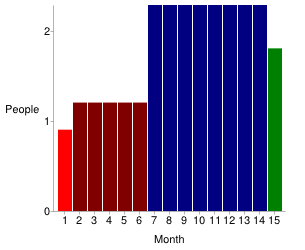
\includegraphics[width=0.7\textwidth]{immagini/chart.png}}
  \caption{Staffing profile}
\end{figure}

\section{Deductions and conclusion}
The COCOMO II estimation reported that there would be needed a total of 14.1 months and 1.7 people making of a total of 26.4 people-month for developing this project. Considering the data reported by the Office of the Chief Financial Officer of the University of California, Berkeley an average of 180 hours per month were spent between Dec. 2014 and Jan. 2015. This makes so a total of 4752 hours-people and 2538 total hours estimated for completing this project. Actually, we spent a total of 445 + 283 hours, divided for each person involved in the project. This is the 15\% of the estimated cost, meaning that this software can be considered as very immature in its development , that the estimation parameters were overrated for the real characteristics of this project and, obviously, that the COCOMO II model is not an exact model of the reality but just an approximated model.